\documentclass[11pt]{article}
%
\usepackage{abstract,amsmath,amssymb,latexsym}
\usepackage{enumitem,epsf}
\usepackage[stable]{footmisc}
\usepackage{fullpage,tikz,float}
\usepackage{caption}
\usepackage[numbers]{natbib}
\usepackage[pdftex,colorlinks]{hyperref}
\usepackage{array, booktabs}
\usepackage{graphicx}
\usepackage{colortbl}
\usepackage{wrapfig}
\usepackage[TS1,T1]{fontenc}


\newcommand{\foo}{\makebox[0pt]{\textbullet}\hskip-0.5pt\vrule width 1pt\hspace{\labelsep}}


% locally defined macros
\usepackage{macros}

%%%%%%%%%%%%%%%%%%%%%%%%%%%%%%%%%%%%%%%%%%%%%%%%%%%%%%%%%%%%%

% Use the following for revealing TODOs and appendices
% Options are: \draftfalse or \drafttrue
\newif\ifdraft
\draftfalse

%%%%%%%%%%%%%%%%%%%%%%%%%%%%%%%%%%%%%%%%%%%%%%%%%%%%%%%%%%%%%

\title{
 \begin{minipage}[c]{1.05\textwidth}
 	\centerline{Massively Multiagent Inverse Reinforcement}
 	\centerline{ Learning in Open-world Environments}
 \end{minipage}
}

\author{
	\vspace{1cm}
	William H. Guss\thanks{Carnegie Mellon University, Machine Learning Department.}\\[-1cm]
	wguss@cs.cmu.edu \and
	Ruslan Salakhutdinov\footnotemark[1] \\
	rsalakhu@cs.cmu.edu
}

\begin{document}

\maketitle
\thispagestyle{empty}


\setcounter{page}{1}



\vspace{-10pt}
\belowcaptionskip -21pt
\begin{wrapfigure}{r}{0.48\textwidth}
\centering 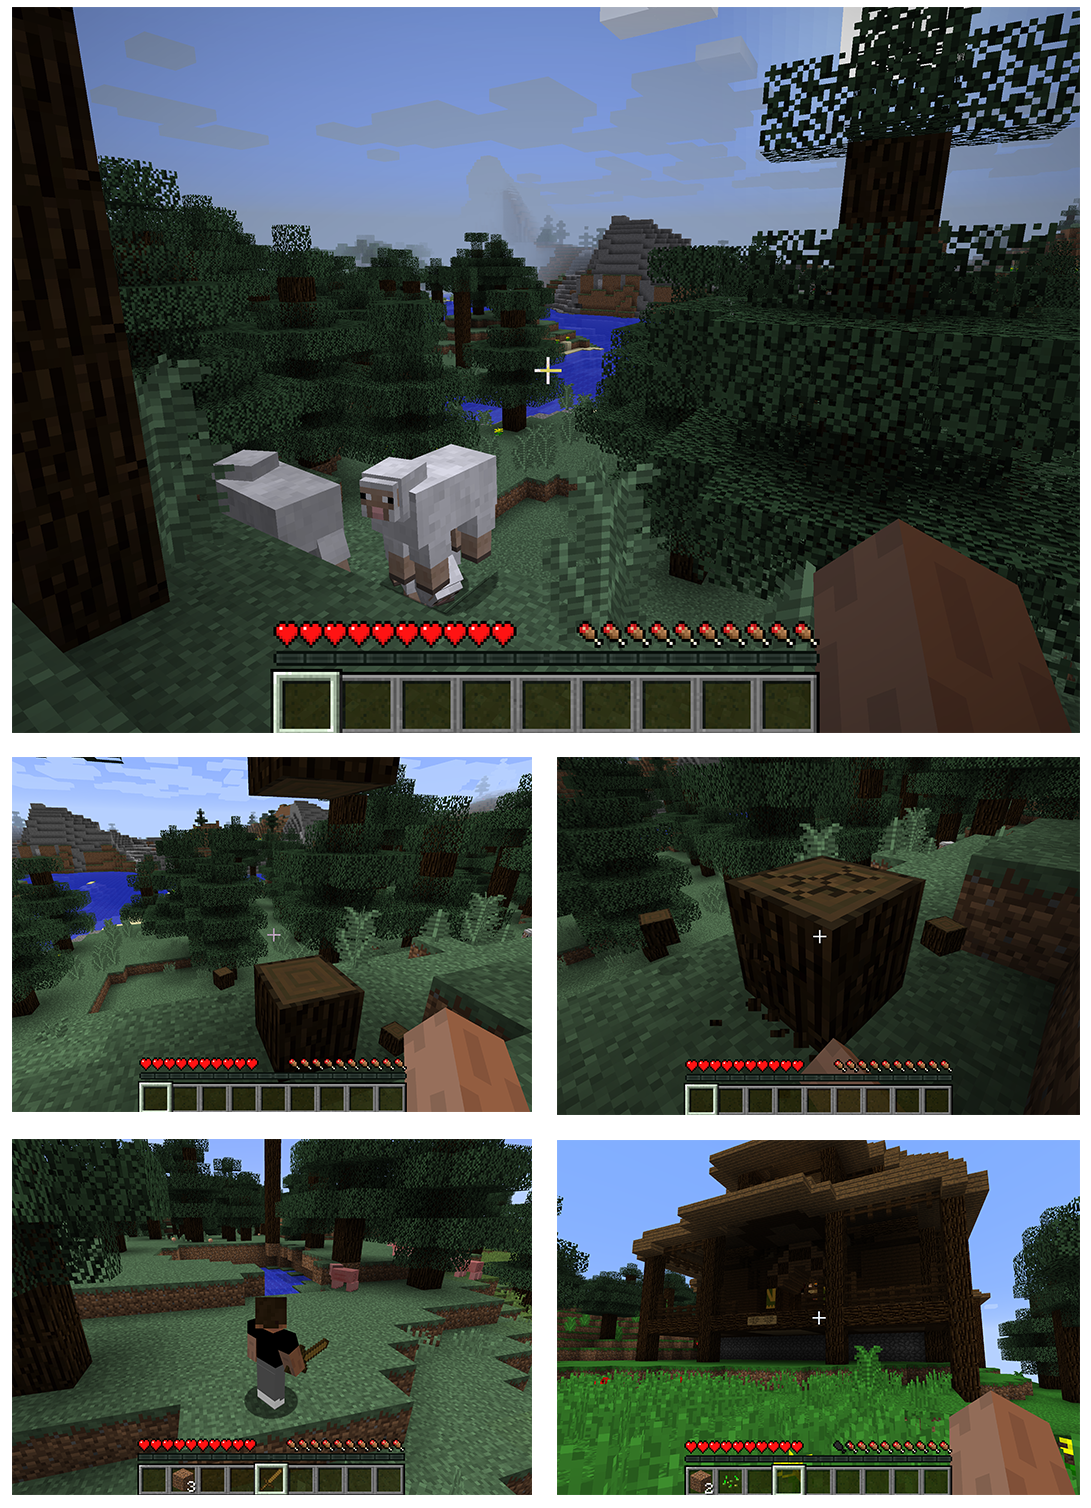
\includegraphics[width=0.47\textwidth]{mc_combined.png}
\caption{An example of different states in Minecraft, such as resource gathering, environment discruction, combat, building, and mining.}
\end{wrapfigure}

\section{Introduction}

Over recent years inverse reinforcement learning (IRL) has revolutionized the state of the art in apprenticeship learning, cooperative and adversarial modeling, and the modeling of intent in human and animal behaviour\todo{cite}. At its core, IRL solves the problem of learning expert policies indirectly: in direct juxtaposition to behavioral cloning IRL learns the reward function of an expert agent and then produces a policy which maximizes that reward. In this regime, the resultant policy is often far more interpratable, robust, and sample efficient than that of behavioural cloning. 

Mechanically, inverse reinforcement learning is optimal not only for cloning expert policies in applications where thousands if not millions of demonstrations are not possible, but also as a substitute for traditional reinforcement learning when exploration is extremely expensive. For example, in robotic manipulation tasks, where typical $\epsilon$-greedy exploration polices would result in potential damage to the robot, apprenticeship learning via IRL is a powerful alternative. Furthermore, by learning the reward function directly, IRL is an effective, interpritable forecasting mechanism in tasks such as epidimiological modeling, traffic prediciton, and first person activity forecasting.\todo{cite}


Despite its numerous applications and avantages, IRL is an underconstrained optimzation problem; in particular, there are potentially inifinitely many reward functions which explain an expert policies behaviour. To see this formally, let $(S,A,T,\gamma,D)$ be a rewardless Markov deciion process (MDP) with state space $S$, action space $A$, state-to-state transition function $T$, $\gamma$ some marginal utility discount, and $D$ an initial state distribution. Given some expert policy $\pi^*(a | s )$, where $a \in A, s \in S$, inverse reinforcement learning aims to find a reward function $R: S \times A \to \mathbb{R}$ such that 
\begin{equation}
	\pi^* = \arg \max_{\pi} \mathbb{E}\left[\sum_{t=1}^\infty \gamma^t  R(s_t, a_t)\right]
\end{equation}
where $s_t \sim T(s_{t-1}, a_{t-1}), a_t \sim \pi(\cdot | s_t),$ and $s_0 \sim D.$ In this setup, it is clear that degenerate reward functions such as $R = 0$ suffice in explainig $\pi^*.$ Constraining the space of candidate reward functions has therefore become central problem in inverse reinforcement learning. 

% \todo{Previous research on reward constraints, plus hook.}


% \todo{Provide a slightly more formal perspectrive to motivate why these methods could be interesting?}


% \todo{Introduce the problem statement, what is the problem of massively multiagent hierarchical reinforcement learning in open-world environments and why would this be pertinent.}

% \todo{Introduce the implications of solving the MMHIRL problem in open-world environments, potentially reference the taxi problem.}


\section{Our Approach}

In this project we propose a novel approach the problem of reward space regularization by leveraging the statistical power of large scale massively multiexpert policy trajectories in open-world environments. In particular, we will develop new algorithms which allow inverse reinforcement learning to utilize policy rollouts from multiple distinct experts whose reward functions are assumed to be samples from some continuously parameterized manifold of reward functions. Thereafter, we will develop a cloud-based massively multiplayer environment to record a sufficiently rich dataset of expert trajectories in Minecraft, an open-world game with inductively ambiguous reward structures. Finally, we will apply the foregoing methods to train deep reinforcement learning agents using different player reward functions sampled from the learned reward space. In addition to being introduced to the envrionment, these agents will serve as a benchmark for the efficacy of the inverse reinforcement learning procedure evaluated by several metrics.\\


\noindent\textbf{Multi-reward Inverse Reinforcement Learning}. In contrast to existing methods, our proposed approach, multi-reward inverse reinforcement learning (MIRL), exploits the following fact: although in multiagent open-world environments, each individual agent is governed by its own reward function, between any two agents their respective rewards are similar; that is, there is a semi-continuous parameterization of the space of reward functions over some reasonable population of agents in an open-world environment. This assumption leads to a powerful regularization scheme wherein degeneracy of a particular agents reward function is penalized as that agent's reward must be $\epsilon$-sufficient for explaining the actions of another similar but distinct agent. \\

\noindent \textbf{Open-world environment.} To collect sufficiently realistic and open-world samples for MIRL we will develop a custom extension to the multiplayer version of Minecraft. Minecraft, see Figure 1, is a survival-based sandbox game wherein players are given full agency to build, destroy, and explore their environment. In addition to the huge state space, in an online setting players can fight or collaborate in constructing various buildings, cities, and communities. Generally speaking there is no particular goal, score, or objective\footnote{With the exception of experience, which will be used as a metric for  the evaluation of MIRL.} which governs players actions; that is, each player defines their own reward structure and the game is as seemingly open-world as the real world.

Over the duration of the project, we will host a minecraft server which records every players screen and actions and collates this data into a coherent data-store. At scale we anticipate the server will host more than 1000 unique players generating 30 frames per second each. The resulting dataset of player trajectories will be the largest of its kind. As aforementioned, we will also develop tooling for the introduction of learned agents into the environment with which players will continually interact.


% \todo{To solve the problem of MMHIRL we will introduce methods which take advantage of the local connectedness of parameterized policy and reward space.}

% \todo{}


\subsection{Experiments}

The proposed project will consist of multiple experiments for testing the efficacy of the MIRL. 

1. \textbf{Single Player Expeirment.} Using the existing dataset, we will compare several techniques including inverse reinforcement learning, behavioral cloning, DAGGer, and weakly supervised reinforcement learning. After training apprentice agents using the foregoing methods, each will be tested in a single-player instantiation of the minecraft environment and studied observationally and empirically. In particular for the resultant MIRL policies, we will test not only the efficacy of the average policy sampled from the reward space, but also that of the interpolation of several policies via transport in the original domain. Each agent, regardless of algorithm, will be measured according to number of experience points gained, number of deaths, total distance moved, square area explore, and other such similar metrics. Note that although these metrics exists, none of them are sufficient to compose a reward function for an individual player of the game.

2.\textbf{ Multiplayer Experiment.} The strategy of a large portion of policies in an open-world setting relies on communication and collaboration. Therefore, an extension of the single-player experiment will introduce multiple agents learned as a result of MIRL and the foregoing baseline methods. In this experiment $N$ agents will be spawned in the same location and the methods compared according ot their ability to elicit collaboration; i.e., average distance between different agents minimized, building blocks placed in proximity to one another, etc. Additionally the same metrics as suggested in the single player experiment will be used to establish the efficacy of a group of agents spawned using a particular algorithm.

3. \textbf{Large Scale Action Forecasting}. Lastly, as aforementioned, when successful inverse reinforcement learning is a powerful tool for action/trajectory forecasting. Therefore we will measure the efficacy of MIRL incomparison to standard IRL methods  





\bibliographystyle{plainnat}
\bibliography{bib}

\end{document}
